\documentclass[letterpaper]{article}

\usepackage{aaai}
\usepackage{amsmath}
\usepackage{amssymb}
\usepackage{amsthm}
\usepackage{courier}
\usepackage{graphicx}
\usepackage{helvet}
\usepackage{times}

\newtheorem{definition}{Definition}
\newtheorem{example}{Example}
\newtheorem{formula}{Formula}
\newtheorem{problem}{Problem}

%\setlength\parindent{0pt}
\frenchspacing

\setlength{\pdfpagewidth}{8.5in}
\setlength{\pdfpageheight}{11in}

\pdfinfo{
/Title Rough Set Semantics for Identity management on the Web
/Author Wouter Beek, Stefan Schlobach, Frank van Harmelen}
\setcounter{secnumdepth}{0}

\begin{document}

\title{Rough Set Semantics for\\Identity management on the Web}
\author{Wouter Beek, Stefan Schlobach, Frank van Harmelen}
\maketitle
\begin{abstract}
\begin{quote}
\end{quote}
\end{abstract}

\section{Introduction}

Identity relations are at the foundation of the Linked Open Data initiative and on the Semantic Web in general. They allow the interlinking of alternative descriptions of the same thing. However, the traditional notion of identity (owl:sameAs) is often problematic, e.g. when objects are considered the same in some contexts but not in others. The standing practice in such cases is to use weaker relations of relatedness (e.g. skos:related). Unfortunately, this limits reasoners in drawing inferences. 

We propose a method that treats a given identity relation as a collection of indiscernability pairs, assigning meaning to such relations in terms of shared properties/values. Reflexivity, symmetry and (in some cases) transitivity are preserved under indiscernability, allowing reasoners to infer new results.

Reinterpreting identity in this way allows the calculation of upper and a lower bounds, turning crisp identity into rough indiscernability, based on the well-understood rough-set semantics. These rough sets can be used to provide automated assistance for finding false positive and false negative errors for existing linksets.

In a series of experiments we show that this method can indeed be used to improve on linksets that are the result of state of the art automated alignment mappings.

\subsection{Previous work}

\subsection{Research goals}

First goal: In a linkset the identity pairs all look the same. We want to characterize subsets of a linkset based on the identity conditions that we can extrapolate from the data. In this way we can assign meanings to sets of indentity pairs.

Second goal: Based on an exiting identity relation, and using concepts from rough set theory, we can define an approximation of that identity relation. Based on this approximation semantically moticated suggestions can be given for extending and/or limiting the identity relation.

Third goal: We wamt to establish the quality of an identity relation in quantitative means, i.e. in semantic terms.

\section{Shared properties \& shared shared properies}

For a given identity relation there may be different subrelations that we can identify in terms of the semantics of the graph. For instance, in the merged IIMB graph there are some identical resources that share the property \verb|IIMBTBOX:spoken_in|, while other pairs share the property \verb|IIMBTBOX:form_of_government|. The set of pairs of resources that are spoken in the same language may even be disjoint from the set of pairs of resource that have the same form of government.

Note that we are not only interested in the properties that resources share with one other (e.g., where they are spoken or which form of government they have), but also in which resource pairs share the same sharing properties. We can thus identify subsets of an identity relation based on differences in the sets of predicates relative to which they are discernable.

We say that two resources are indiscernible ($IND(P)$, definition \ref{def:unary_indiscernability}) in case they share the same properties. We say that two resource pairs are indiscernible ($IND(P^*)$, definition \ref{def:binary_indiscernability}) in case both pairs are indiscernible for the same $P \subseteq \mathcal{P}(P_G)$.

\begin{definition}[Indiscernability]
\begin{align}
IND(P) = \{
  \langle x, y \rangle \in S_G^2
\  \vert \ 
  \forall a \in P(a(x) = a(y))
\}
\label{def:unary_indiscernability}
\\
IND(P^*) \  = \  \{
    \langle
      \langle x_1, y_1 \rangle,
      \langle x_2, y_2 \rangle
    \rangle \in (S(G)^2)^2
  \  \vert \ 
\\
    \forall P \in P^*(P(x_1, y_1) = P(x_2, y_2))
  \}
\label{def:binary_indiscernability}
\end{align}
\end{definition}

For a given set of identity pairs, there may be multiple pairs that have the same shared properties. These sets of predicates that are shared across resource pairs are considered to give a description of a specific subrelation of the identity relation. In figure \ref{fig:indiscernibility_example} the subrelation $\{ \langle a, c \rangle, \langle b, c \rangle \}$ is characterized by $\mathcal{P}(\{ P \})$.

\begin{figure}
\caption{This figure contains four constants, represented by nodes and annotated with the properties $P$, $Q$, and $R$ that apply to them. It also contains six pairs, represented as edges between the nodes (reflexive pairs are not shown). The edges are drawn inside squares that represent the indiscernability sets to which they belong. For instance $\langle a, b \rangle$ and $\langle a, c \rangle$ belong to the same indiscernability set $\mathcal{P}(P)$.}
\label{fig:indiscernibility_example}
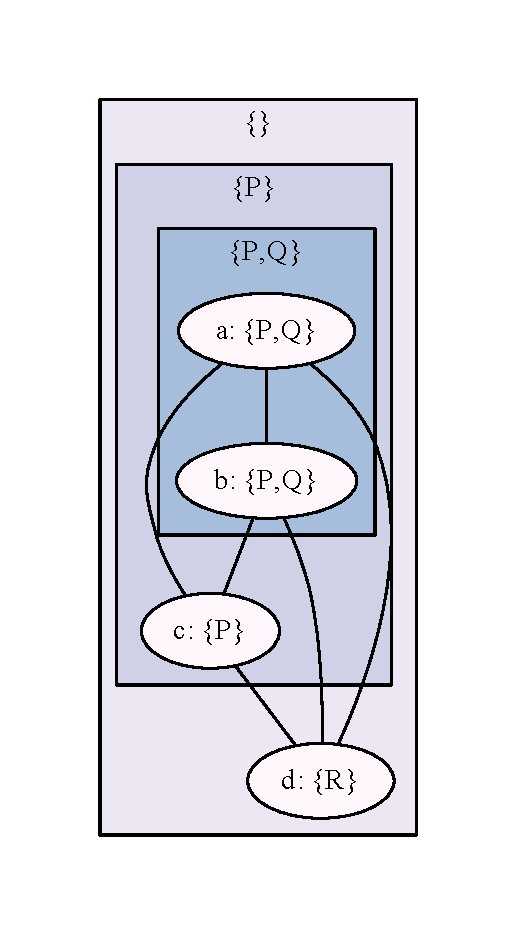
\includegraphics{indiscernibility_example}
\end{figure}

\section{Approximation}
\label{sec:approximation}

In our approach we approximate the identity relation by using rough set theory [REF] to represent approximations of the full set of identity pairs. We assume that an RDF graph $G$ and a binary relation $\approx$ are given in advance.\footnote{For our approch it is not necessary to pose additional restrictions on the binary relation. In practice this will be either a linkset relating subgraphs of $G$ to each other, or a set of alignments created by an ontology mapping tool.}

As the domain of our rough set approach we take the Cartesian product of the resources that occur in the subject position of some triple in the graph $S_G$. As the set of relations\footnote{Relations are usually called attributes in rough set theory, and they are functions that map to an arbitrary set of value labels. We only consider functions that map onto the set of Boolean truth values.} we take the powerset of those resources that occur in the predicate prosition of some triple in the graph $P_G$. This means that we have a big number of primitives to work with (a quadratic number of constants; an exponential number of relations).

For an arbitrary binary relation $\approx$ we can define a higher (\ref{def:higher_approximation}) and a lower (\ref{def:lower_approximation}) approximation of that relation. Relation $\mathbb{R}$ characterizes a similarity metric between resource pairs. The intuition behind these definitions is that pairs that are similar to $\approx$-pairs should be in the higher approximation. 

\begin{definition}[Higher \& lower approximation]
\begin{align}
x \overline{\approx} y \  & \iff & \ 
  \exists u,v (
      \mathbb{R}(\langle u, v \rangle, \langle x, y \rangle)
    \land
      u \approx v
  )
\label{def:higher_approximation}
\\
x \underline{\approx} y \  & \iff & \ 
  \forall u,v (
      \mathbb{R}(\langle u, v \rangle, \langle x, y \rangle)
    \rightarrow
      u \approx v
  )
\label{def:lower_approximation}
\end{align}
\end{definition}

Since we want to stay close to the traditional notion of identity, we choose the indiscernability relation as our $R$.


\subsection{Indiscernability}

As in rough set theory, we define indiscernability as a set of pairs for which it is impossible to show the distinction.

Note that we do not define indiscernability on the level of resources, but on the level of pairs of resources (definition \ref{def:binary_indiscernability}. This allows us to define a rough set of pairs that is based on the given identity relation $\approx$.\footnote{As noted earlier, this could be done based on \emph{any} binary relationship, regardless of whether or not it is assumed to consitute an identity relation.}

For every set of predicates $P^*$ (i.e., subset of $\mathcal{P}(P(G))$) we can define the binary indiscernability relation \ref{def:binary_indiscernability}.

\begin{definition}[Higher \& lower approximation]
\label{def:higher_lower_approximation}
\begin{align}
y \in [x]_H \  \text{iff} \  \exists [u]_{\approx} (
    \vert [u]_{\approx} \vert > 1
  \land
    \mathbb{P}([u]_{\approx}) = \mathbb{P}(\{ x, y \})
  ) \\
y \in [x]_L \  \text{iff} \  \forall S \subseteq D (
    (\vert S \vert > 1 \land \mathbb{P}(S) = \mathbb{P}(\{ x, y \}))
  \rightarrow
    \exists s \in D (S = [s]_{\approx})
  )
\end{align}
\end{definition}

\subsection{Hypotheses}

The quality of a linkset is inversely correlated with the size of the boundary

\section{Experimental results}

\section{Conclusion}

\end{document}

